\documentclass[czech, kiv, ba, he, iso690auyr, pdf]{fasthesis}

\usepackage{url}
\usepackage{enumitem}

\title{Implementace modulu pro import údajů RÚIAN}
\author{Martin}{Schön}{}{}
\supervisor{Martin Bíkl, Ing. Petr Přibyl, Ing. Martin Zíma Ph.D.}
\stagworkid{100718}
\assignment{figures/zadani.pdf}
\signdate{31}{12}{2024}{V Plzni}
\addbibresource{bib.bib}
\abstract{Text abstraktu v~jazyce práce, tj. zde česky.}
{The abstract text in a secondary language, here in English.}
\keywords{
    RÚIAN -- Registr územní identifikace adres a nemovitostí\\
    VFR  -- Výměnný formát RÚIAN
}
\acknowledgement{Text poděkování.}

\begin{document}
\frontpages[tm]
\tableofcontents
%---------------------------------------------------------------------------
\chapter{Úvod}
Problematika správy prostorových dat a~jejich synchronizace mezi různými systémy 
nabývá na významu s~rostoucí digitalizací státní správy a~soukromých sektorů. 
Jedním z~klíčových zdrojů těchto dat v~České republice je Registr územní identifikace, 
adres a~nemovitostí (RÚIAN), který poskytuje rozsáhlé a~aktuální informace o~územních 
objektech, adresách a~dalších klíčových entitách. Efektivní využití dat z~RÚIAN vyžaduje 
nejen jejich přístup prostřednictvím datových služeb, ale také robustní řešení pro mapování, 
konfiguraci a~synchronizaci datových struktur.

Cílem této bakalářské práce je analyzovat datové schéma registru RÚIAN a~možnosti získávání 
dat prostřednictvím nabízených datových služeb. Dále bude provedena analýza a~návrh konfiguračního 
řešení, které umožní nastavit úroveň přenášených územních objektů a~cílové databázové struktury. 
V~rámci práce bude navržena a~implementována aplikace, která umožní pravidelnou synchronizaci dat 
z~veřejné databáze RÚIAN do cílových databázových struktur s~podporou databází Oracle, 
Microsoft~SQL Server a~PostgreSQL. Aplikace bude schopna provádět synchronizaci kompletních datových 
sad i~přírůstkových změn podle zadané konfigurace.

\chapter{RÚIAN}
\section{Co je to RÚIAN}
Jedná se o~státní informační systém v~České republice, který obsahuje 
informace o~adresách, budovách, parcelách a~dalších objektech. Systém 
je spravován Českým úřadem zeměměřickým a~katastrálním (ČÚZK). 
Data jsou využívána v~mnoha oblastech, například v~urbanistickém plánování, 
geodézii, nebo při správě nemovitostí. Jednotlivé prvky jsou zobrazovány na~mapách 
státního mapového díla a~digitální mapě veřejné správy. 

Data z~RÚIAN jsou veřejně dostupná a~lze je získat z~webové služby na~adrese 
\url{https://vdp.cuzk.cz/vdp/ruian}. V~této aplikaci je možné vyhledávat konkrétní 
prvky nebo ověřit jejich existenci. Data jsou poskytována ve formátu XML a~lze je 
automaticky stahovat pomocí API. Tyto informace jsou pravidelně aktualizovány, 
což zajišťuje jejich aktuálnost a~přesnost.

\section{VFR}
Výměnný formát RÚIAN je služba poskytující data.
Je možné stahovat data dle zadaných formátů: Standardní, Historický a~Speciální.
Dále je možné si vybrat přírůstková data nebo úplnou kopii.
Každý formát obsahuje dodatečně parametry, které je možné nastavit.
Data z~VFR jsou ve~formátu XML.
Každý element obsahuje atributy, které obsahují informace o~dané entitě (Tabulce).
\newpage
\begin {itemize}
    \item \textbf{Standardní} -- obsahuje úplná nebo přírůstková data.
    \begin {itemize}
        \item Časový rozsah: Přírůstky od~data / Úplná kopie
        \item Územní prvky: Stát až~ZJS / Obec a~podřadné
        \item Datová sada: Základní / Kompletní
        \item Výběr z údajů: Základní údaje / Gen. hranice, Originální hranice, Vlajky a~znaky
        \item Územní omezení: ČR / Kraj (VÚSC) / ORP / Obec
    \end {itemize}
    \item \textbf{Historický} -- obsahuje historická data.
    \begin {itemize}
        \item Časový rozsah: Přírůstky od~data / Úplná kopie
        \item Územní prvky: Stát až~ZJS / Obec a~podřadné
        \item Územní omezení: ČR / Kraj (VÚSC) / ORP / Obec
    \end {itemize}
    \item \textbf{Speciální} -- obsahuje speciální data.
    \begin {itemize}
        \item Časový rozsah: Přírůstky od~data / Úplná kopie
        \item Výběr z~údajů: Číselníky / Vazby / Vazby a číselníky
        \item Kategorie: Všechny / Geodetické body / Nerostné bohatství
    \end {itemize}
\end {itemize}

\section{Tabulky}
Data z~RÚIAN jsou rozdělena do několika tabulek.
Jak je vidět na~obrázku~\ref{fig:ruian_tables}, každá tabulka obsahuje jiné informace.
Některé tabulky obsažené v~RÚIAN jsou nepotřebné. 
Příkladem může být tabulka \textit{Stát}, která obsahuje informace o~státu Česká republika.
Ovšem RÚIAN obsahuje pouze informace o~České republice, tudíž tato tabulka je nadbytečná.
Které tabulky budou zpracovány a~které budou ignorovány, záleží na~specifikaci 
v~XSD (XML Schema Definition) souborech v~dokumentaci VFR. 
\newpage

\begin{figure}[ht]
    \centering
    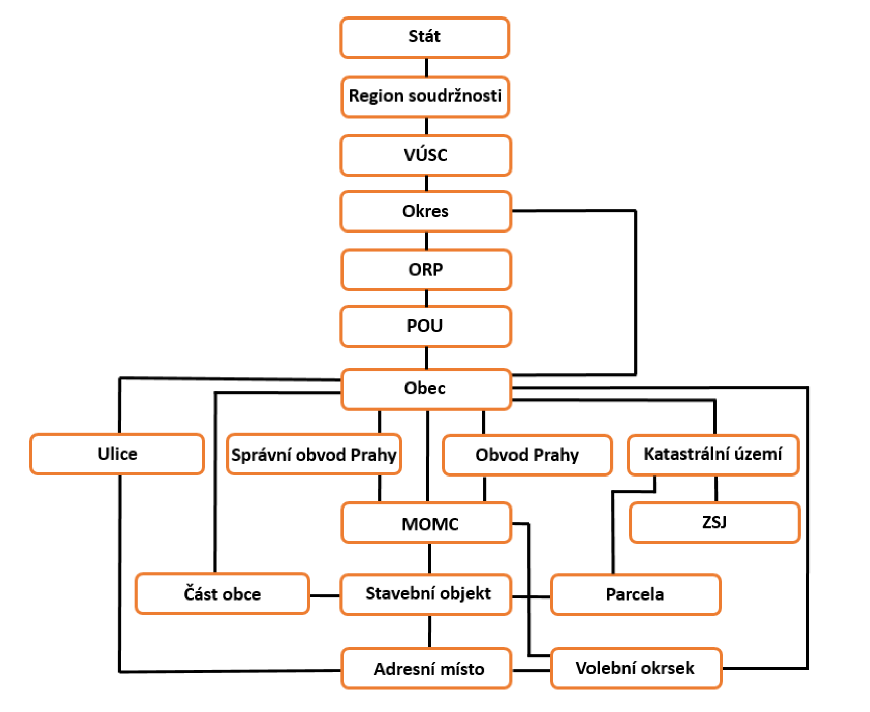
\includegraphics[width=\textwidth]{figures/ruian_tables.png}
    \caption{Tabulky RÚIAN}
    \label{fig:ruian_tables}
\end{figure}


\section{Uložení dat}
Vzhledem k~formátu dat získávaných z~VFR je nezbytné zvolit 
vhodný způsob jejich ukládání, který zajistí efektivní organizaci, správu a~manipulaci s~daty. 
Nejlepší možností se jeví využití relační databáze, která poskytuje robustní nástroje pro 
ukládání dat s~pevně definovanou strukturou a~jejich vzájemné propojení prostřednictvím klíčů.

\chapter{Databáze}
\section{Co je to databáze}
Databáze je softwarový nástroj, který slouží k~efektivnímu ukládání, organizaci a~vyhledávání dat. 
Díky své strukturované povaze umožňuje správu velkých objemů dat a~poskytuje funkcionality pro 
zajištění konzistence, bezpečnosti a~rychlého přístupu k~uloženým informacím.

Databáze lze obecně rozdělit do~dvou hlavních kategorií: \textbf{relační databáze} a~\textbf{Objektové databáze}. 
Každý z~těchto přístupů má své specifické vlastnosti a~je vhodný pro odlišné typy aplikací.

\begin{itemize}
    \item \textbf{Relační databáze}
    \begin{itemize}[itemsep=-1pt]
        \item Data jsou uložena v~tabulkách
        \item Každý řádek tabulky obsahuje jeden záznam
        \item Každý sloupec tabulky obsahuje jeden atribut
        \item Vztahy mezi tabulkami jsou definovány klíči
        \item Využití SQL jazyka
    \end{itemize}
    Relační databáze jsou vhodné pro strukturovaná data, která mají pevnou strukturu.
    Jedná se o~nejčastěji používaný typ databáze.

    \item \textbf{Objektové databáze}
    \begin{itemize}[itemsep=-1pt]
        \item Data jsou uložena jako objekty
        \item Každý objekt obsahuje atributy a~metody
        \item Vztahy mezi objekty jsou definovány referencemi
        \item Využití objektově orientovaného jazyka
    \end{itemize}
    Objektové databáze jsou vhodné pro nestrukturovaná data, která mají složitou strukturu.
    Jedná se o~novější typ databáze, který je vhodný pro moderní aplikace.
\end{itemize}

Jaká je tedy vhodná databáze pro uložení dat z~RÚIAN VFR?
Vzhledem k~tomu, že data z~VFR mají pevnou strukturu a~jsou vzájemně propojena klíči, 
je nejlepší volbou relační databáze. Pro zpracování dat z~RÚIAN VFR je tedy vhodná relační databáze.
Na relační databázi bude třeba vytvořit schéma dle dříve zmíněných tabulek a~zvolení databázového systému.
Pro účely této práce byly zvoleny 3 následující databázové systémy: Microsoft SQL Server, PostgreSQL a~Oracle.

\section{Microsoft SQL Server}
Microsoft SQL Server je relační databázový systém, který vyvinula společnost 
Microsoft a~který se stal jedním z~předních nástrojů pro ukládání, správu a~analýzu dat. 
SQL Server je robustní a~výkonný systém, který nabízí širokou škálu funkcí 
a~možností přizpůsobení pro různé typy aplikací. Díky své dlouhodobé podpoře a~integraci 
s~dalšími produkty společnosti Microsoft, jako je Azure nebo Power BI, je SQL Server 
oblíbenou volbou pro velké a střední podniky.

Edice SQL Serveru zahrnují Standard, Enterprise a~Express, 
které se liší funkcemi a~cenou. Standard Edition je nejčastěji používanou edicí, 
která obsahuje všechny základní funkce a~je vhodná pro většinu aplikací.

SQL Server byl původně navržen výhradně pro Windows, ale od verze SQL Server 2017 je dostupný 
také pro operační systém Linux. Tato multiplatformní podpora zvyšuje jeho použitelnost 
v~různých IT prostředích.
\cite{microsoft_sql_server}

\section{PostgreSQL}
PostgreSQL je open-source relační databázový systém, který je známý svou spolehlivostí, výkonem 
a~rozšiřitelností. Původně byl vyvinut jako alternativa k~proprietárním řešením, jako je SQL Server, 
a~dnes se řadí mezi nejpokročilejší relační databázové systémy na trhu. Díky své otevřené povaze 
a~aktivní komunitě uživatelů a~vývojářů se stal oblíbenou volbou nejen mezi malými firmami, 
ale také ve středních a~velkých organizacích.

PostgreSQL je dostupný zdarma a~podporuje všechny hlavní operační systémy, včetně Windows, Linux a~macOS. 
Tato multiplatformní dostupnost umožňuje snadnou integraci PostgreSQL do různých vývojových prostředí.
\cite{postgresql}

\section{Oracle}
Oracle Database, vyvinutá společností Oracle Corporation, patří mezi přední relační 
databázové systémy na světě. Tento systém je známý svou robustností, vysokým výkonem 
a~schopností zvládat kritické podnikové aplikace a~rozsáhlé datové sady. Oracle Database 
je navržena tak, aby poskytovala spolehlivé a~efektivní řešení pro ukládání, správu 
a~analýzu dat ve velkých i~středních organizacích.

Edice Oracle Database zahrnují Standard Edition, Enterprise Edition a~Express Edition,
které se liší funkcemi a~cenou. Enterprise Edition je nejkomplexnější edicí, která
obsahuje všechny pokročilé funkce a~je vhodná pro velké podniky s~náročnými požadavky.

Oracle Database je kompatibilní s~většinou hlavních operačních systémů, včetně Windows, 
Linux a~Unix. Díky tomu může být nasazena v~různorodých IT prostředích podle požadavků organizace.
\cite{oracle_database}

\section{Komunikace s~databází}
Všechny tři databázové systémy podporují komunikaci pomocí SQL jazyka.
SQL (Structured Query Language) je standardizovaný jazyk pro práci s~relačními databázemi,
který umožňuje vytváření, čtení, aktualizaci a~mazání dat.
Pro komunikaci s~databází je tedy třeba vytvořit SQL dotazy, které budou provádět operace nad daty.

Při implementaci je možné využít knihovny a~frameworky, které usnadňují práci se SQL dotazy, 
jako například JDBC pro Javu, psycopg2 pro Python nebo Active Record v~Ruby. 
Tyto nástroje nabízí přístup k~databázi, které usnadňují složitější operace.

Další možností je využití ORM (Object-Relational Mapping), který umožňuje mapování objektů na~tabulky v~databázi.
Mezi populární ORM nástroje patří Hibernate pro Javu, SQLAlchemy pro Python nebo Entity Framework pro .NET. 
Tyto nástroje umožňují programátorům pracovat s~databází více intuitivním způsobem, například pomocí objektů 
místo přímého psaní SQL dotazů. ORM také usnadňuje správu databázových transakcí a~poskytuje nástroje pro migrace, 
které zajišťují snadnou aktualizaci struktury databáze v~průběhu času.

Pro účely této práce bude využit ORM Hibernate, který umožňuje mapování objektů na~tabulky v~databázi a JDBC pro komunikaci s~databází.

\chapter{Konfigurační soubor}
\section{Co je to konfigurační soubor}
Konfigurační soubor je soubor, který obsahuje nastavení aplikace.
V konkrétním případě se jedná o~nastavení:
\begin{itemize}
    \item Databáze -- Connection string
    \item Zdroj -- Webová služba
    \item Výčet tabulek + mapování
    \item Výčet sloupců tabulek + mapování
    \item Plánovač -- Interval stahování
    \item Vytvoření databáze -- ANO/NE
\end{itemize}
Dále bude třeba vybrat vhodný formát pro konfigurační soubor.

\section{Formát}
Pro konfigurační soubor je možné zvolit několik formátů:
\begin{itemize}
    \item XML(XSD) -- Extensible Markup Language
    \item JSON -- JavaScript Object Notation
    \item YAML -- YAML Ain't Markup Language
\end{itemize}
Bude třeba víceúrovňový formát, který umožní snadné čtení a~zápis.
XML je zbytečně složité a~nepřehledné.
JSON je jednoduchý a~přehledný, ale nepodporuje komentáře.
YAML je jednoduchý a~přehledný, podporuje komentáře, ale je méně rozšířený.
Pro účely této práce byl zvolen formát JSON. \cite{cisco_xml_json_yaml}.

\chapter{Technologie}
Některé technologie pro tuto práci již byly zmíněny (Java, JDBC, Hibernate, Quartz, atd.).
Pro účely této práce budou třeba ještě další technologie, které umožní tvorbu aplikace.

\section{Rest API}
REST API (Representational State Transfer Application Programming Interface) je architektonický 
styl pro návrh webových služeb, který umožňuje snadnou a~efektivní komunikaci mezi klientem a~serverem. 
Tento přístup se stal jedním z~nejrozšířenějších způsobů pro integraci aplikací díky své jednoduchosti, 
flexibilitě a~nezávislosti na platformě. REST API využívá standardní metody protokolu HTTP, jako jsou 
GET, POST, PUT a DELETE, k~provádění různých operací s~daty.

REST API poskytuje ideální prostředí pro implementaci přenosu dat díky své flexibilitě a~schopnosti 
pracovat s~různými datovými zdroji. V~této práci bude kladen důraz na robustnost a~spolehlivost API, 
což zahrnuje zpracování chybových stavů, zabezpečení komunikace (například prostřednictvím HTTPS) 
a~optimalizaci výkonu.
\cite{rest_api}

\section{Spring Framework}
Spring Framework je open-source framework pro vývoj aplikací v~jazyce Java.
V~tomto frameworku bude vytvořena aplikace, která bude vše spojovat dohromady.
Spring Framework obsahuje mnoho modulů, které usnadňují vývoj aplikací, 
jako například Spring Boot, Spring Data, Spring Security, atd.
Pro účely této práce bude využit modul Spring Boot, který umožňuje rychlé 
vytvoření aplikace s~minimální konfigurací.
\cite{spring_framework}

\newpage
\section{Plánovač}
V~popisu, co bude potřebovat konfigurační soubor bylo zmíněno, že~bude třeba určit plánovač.
Co je to plánovač?
Plánovač je nástroj, který umožňuje spouštění úloh v~pravidelných intervalech.
Výhodou plánovače je, že umožňuje automatické spouštění úloh bez nutnosti manuálního zásahu.
Je zde několik možných plánovačů, které lze použít:
\begin{itemize}
    \item Cron -- Unix
    \item Task Scheduler -- Windows
    \item Quartz -- Java
    \item Apache Airflow -- Python
\end{itemize}
Všechny tyto plánovače umožňují spouštění úloh v~pravidelných intervalech.
Pro účely této práce byl zvolen plánovač Quartz, který je napsán v~jazyce Java a 
umožňuje spouštění úloh v~pravidelných intervalech.
Intervaly mohou být nastaveny v~cron notaci, což umožňuje velkou flexibilitu při plánování úloh
(každý den v~3:00, každý týden v~pondělí v~8:00, každý měsíc první den v~12:00 atd.).

\section{Docker}
Docker je open-source platforma pro vývoj, nasazení a~provoz aplikací.
Dále umožňuje vytváření kontejnerů, které obsahují všechny potřebné závislosti pro běh aplikace.
Proč je třeba docker?
Pro každou databázi je třeba vytvořit instanci, která bude obsahovat všechny potřebné tabulky, data 
a~klienta pro komunikaci a~práci s databází. Na~to se hodí docker, který umožňuje vytvoření kontejneru s~databází
a~klientem, který bude obsahovat všechny potřebné závislosti pro běh aplikace.
Dále zde může běžet i~plánovač, který bude spouštět úlohy v~pravidelných intervalech.
\cite{docker}


%---------------------------------------------------------------------------
\appendix
\chapter{První příloha}
\backmatter
\printbibliography
\setbackpageqrcode
\backpage
\end{document}